\section{Experiments}
\label{sec:experiments}
We use the environments introduced in \citet{plappert2018multi} for our experiments.
Broadly the environments fall in two categories, Fetch and Hand tasks.
Our results show that learning is possible across all environments
without the requirement of goal-reward.

The Fetch tasks involve a simulation of the Fetch robot's 7-DOF robotic arm. The four tasks are Reach, Push,
Slide and PickAndPlace.
In the Reach task the arm's end-effector is tasked to reach the a particular 3D coordinate. 
In the Push task a block on a table needs to be pushed to a given point on it.
In the Slide task a puck must be slid to a desired location.
In the PickAndPlace task a block on a table must be picked up and moved to a
3D coordinate.

The Hand tasks use a simulation of the Shadow dexterous hand to manipulate objects of
different shapes and sizes. These tasks are HandReach,
HandManipulateBlockRotateXYZ, HandManipulateEggFull and HandManipulatePenRotate.
In HandReach the hand's finger tips need to reach a given configuration.
In the HandManipulateBlockRotateXYZ, the hand needs to rotate a cubic
block to a desired orientation.
For HandManipulateEggFull repeats this orientation tasks with an egg.
To HandManipulatePenRotate does so with a pen.

Snapshots of all these tasks can be found in Figure~\ref{fig:envs}. Note that
these tasks use joint angles, not visual input.


\subsection{Metrics}
Similar to prior work, we evaluate all experiments on two metrics: the success
rate and the average distance to the goal. The success rate is defined as the
fraction of episodes in which the agent is able to reach the goal within a
pre-defined threshold region.
% $\frac{1}{E}\sum_{e,t} \mathbbm{1}_{\|\goal_t - \goal^*\|_2 < \epsilon}$.
The metric \emph{distance of the goal} is the euclidean distance between
the achieved goal and the desired goal in meters.
% $\|\goal_t - \goal^*\|_2$.
These metrics are plotted against a standard progress measure, the
number of training epochs, showing
comparable results of our method to the baselines.

To emphasize that our method does not require goal-reward
and reward re-computation, we plot these metrics against another
progress measure, the number of reward computations used during
training. This includes both the episode rollouts and the reward recomputations
during HER sampling.

%
\begin{figure}%
  \def\frac{0.24}
  \rotatebox{90}{\hspace{2em}\color{blue}{\tiny Fetch Reach}}%
  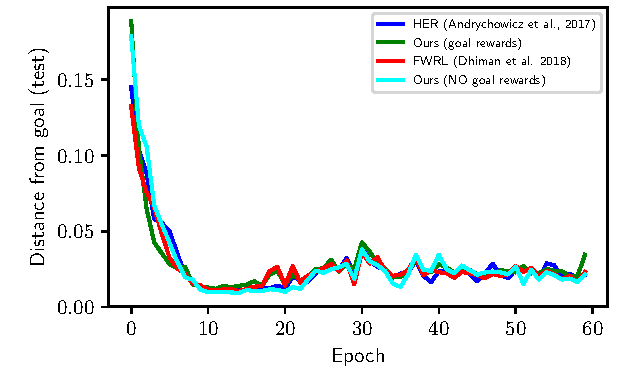
\includegraphics[width=\frac\columnwidth]{media/res/6efc1de-path_reward_low_thresh_chosen-FetchReachPR-v1-dqst/epoch-test/ag_g_dist.pdf}%
  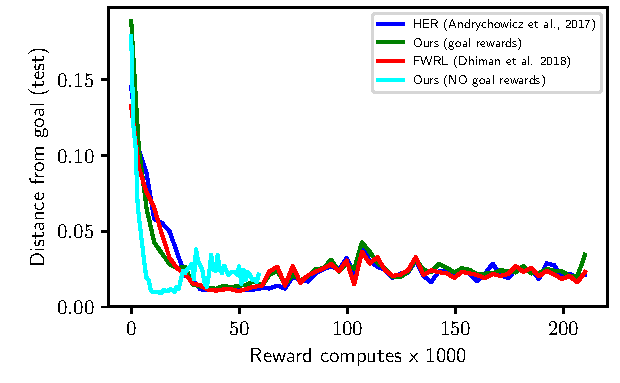
\includegraphics[width=\frac\columnwidth]{media/res/6efc1de-path_reward_low_thresh_chosen-FetchReachPR-v1-dqst/reward_computes-test/ag_g_dist.pdf}%
  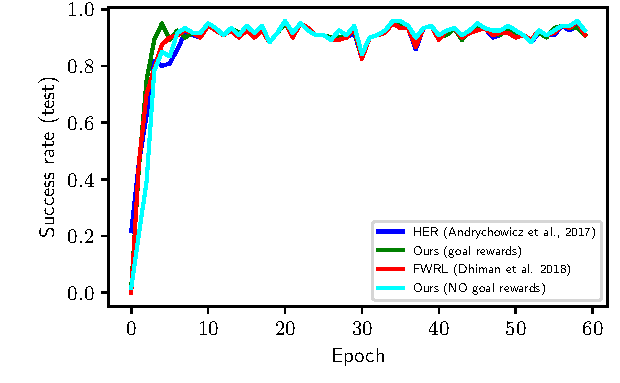
\includegraphics[width=\frac\columnwidth]{media/res/6efc1de-path_reward_low_thresh_chosen-FetchReachPR-v1-dqst/epoch-test/success_rate.pdf}%
  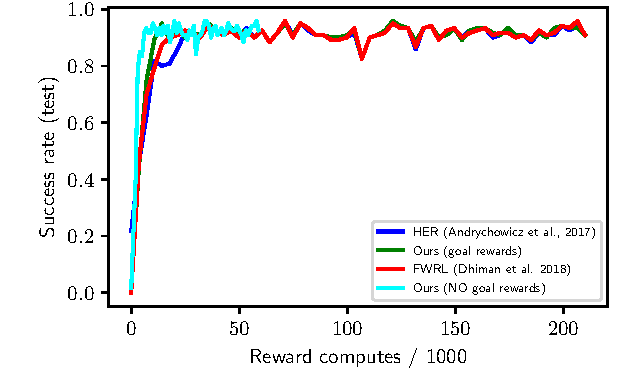
\includegraphics[width=\frac\columnwidth]{media/res/6efc1de-path_reward_low_thresh_chosen-FetchReachPR-v1-dqst/reward_computes-test/success_rate.pdf}\\
  \rotatebox{90}{\hspace{2em}\color{blue}{\tiny Fetch Push}}%
  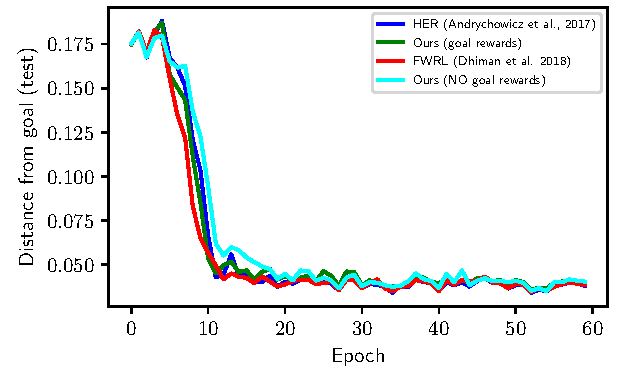
\includegraphics[width=\frac\columnwidth]{media/res/6efc1de-path_reward_low_thresh_chosen-FetchPushPR-v1-dqst/epoch-test/ag_g_dist.pdf}%
  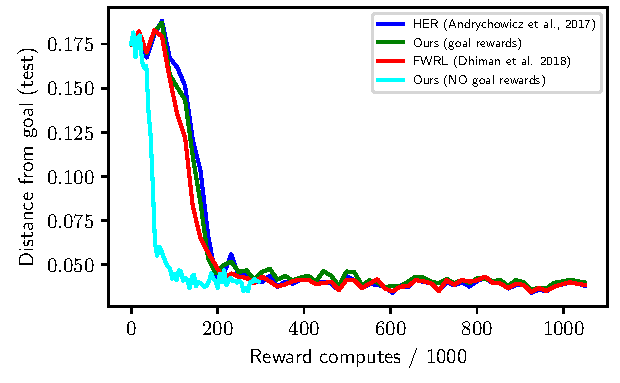
\includegraphics[width=\frac\columnwidth]{media/res/6efc1de-path_reward_low_thresh_chosen-FetchPushPR-v1-dqst/reward_computes-test/ag_g_dist.pdf}%
  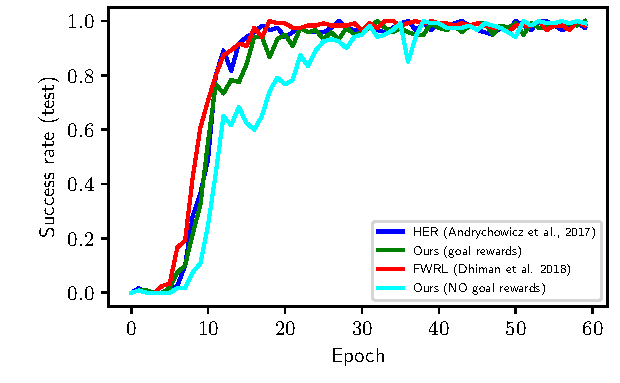
\includegraphics[width=\frac\columnwidth]{media/res/6efc1de-path_reward_low_thresh_chosen-FetchPushPR-v1-dqst/epoch-test/success_rate.pdf}%
  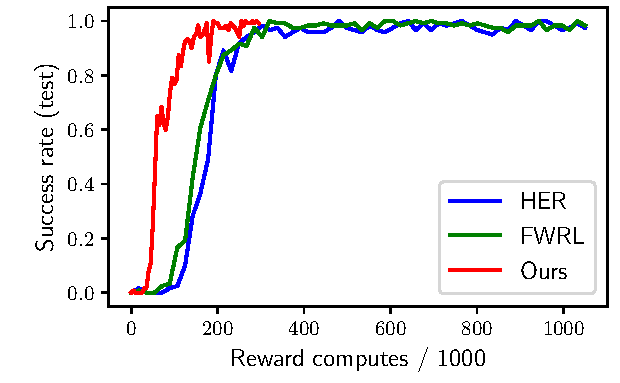
\includegraphics[width=\frac\columnwidth]{media/res/6efc1de-path_reward_low_thresh_chosen-FetchPushPR-v1-dqst/reward_computes-test/success_rate.pdf}\\
  \rotatebox{90}{{\tiny\hspace{1em} \color{blue}{Fetch Pick And Place}}}%
  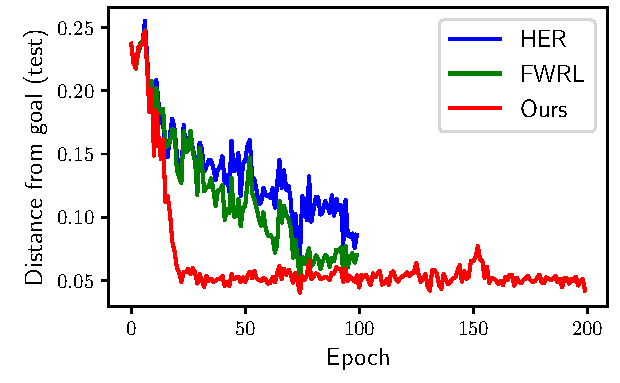
\includegraphics[width=\frac\columnwidth]{media/res/6efc1de-path_reward_low_thresh_chosen-FetchPickAndPlacePR-v1-dqst/epoch-test/ag_g_dist.pdf}
  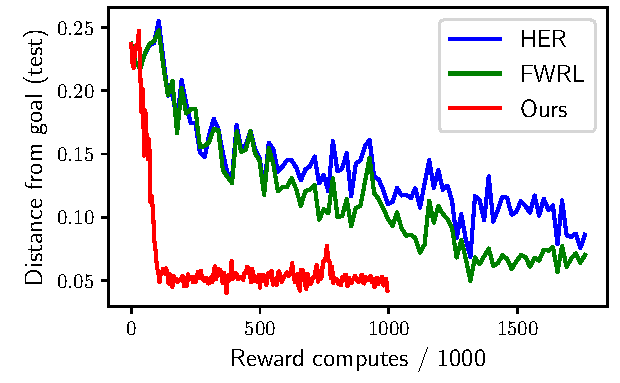
\includegraphics[width=\frac\columnwidth]{media/res/6efc1de-path_reward_low_thresh_chosen-FetchPickAndPlacePR-v1-dqst/reward_computes-test/ag_g_dist.pdf}%
  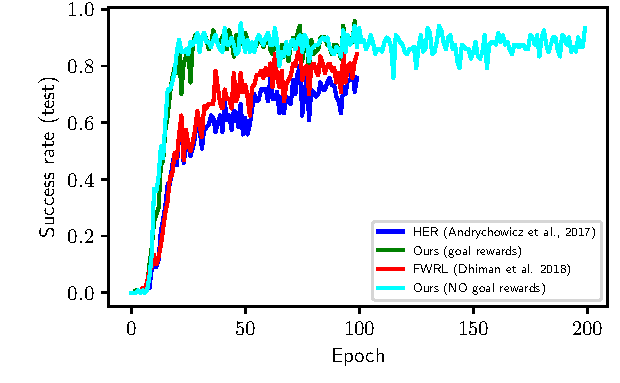
\includegraphics[width=\frac\columnwidth]{media/res/6efc1de-path_reward_low_thresh_chosen-FetchPickAndPlacePR-v1-dqst/epoch-test/success_rate.pdf}%
  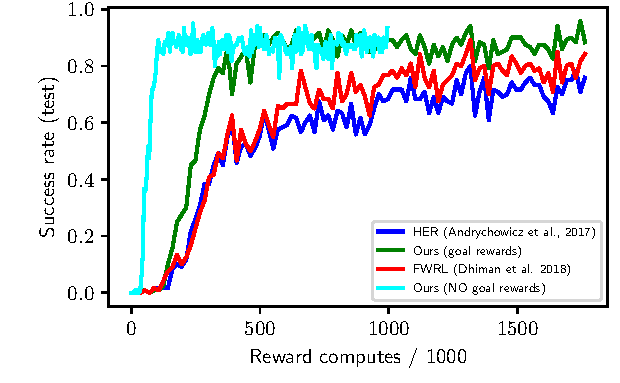
\includegraphics[width=\frac\columnwidth]{media/res/6efc1de-path_reward_low_thresh_chosen-FetchPickAndPlacePR-v1-dqst/reward_computes-test/success_rate.pdf}\\
  \rotatebox{90}{\tiny\hspace{2em}\color{blue}{Fetch Slide}}%
  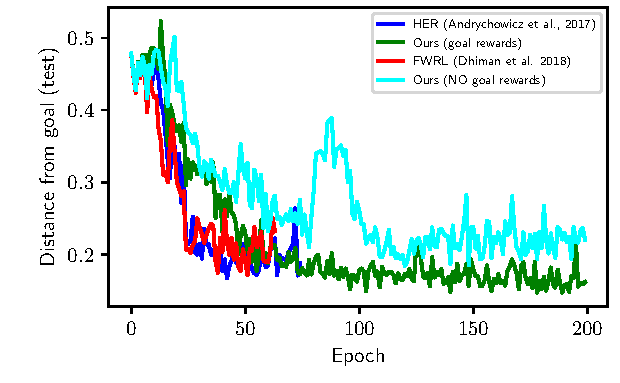
\includegraphics[width=\frac\columnwidth]{media/res/6efc1de-path_reward_low_thresh_chosen-FetchSlidePR-v1-dqst/epoch-test/ag_g_dist.pdf}
  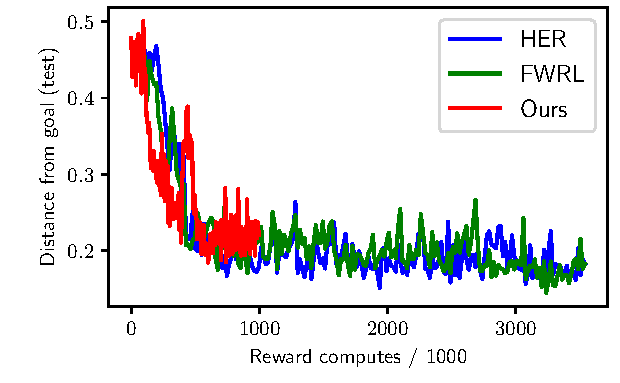
\includegraphics[width=\frac\columnwidth]{media/res/6efc1de-path_reward_low_thresh_chosen-FetchSlidePR-v1-dqst/reward_computes-test/ag_g_dist.pdf}%
  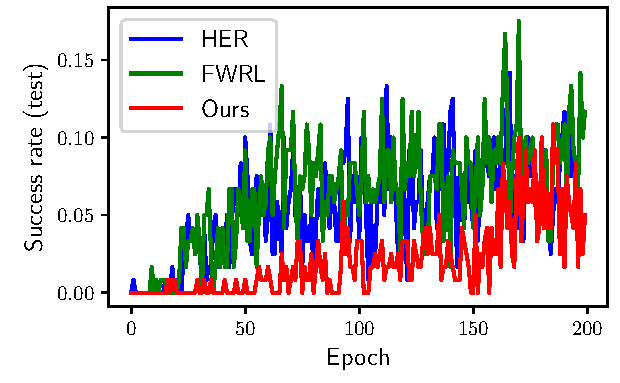
\includegraphics[width=\frac\columnwidth]{media/res/6efc1de-path_reward_low_thresh_chosen-FetchSlidePR-v1-dqst/epoch-test/success_rate.pdf}%
  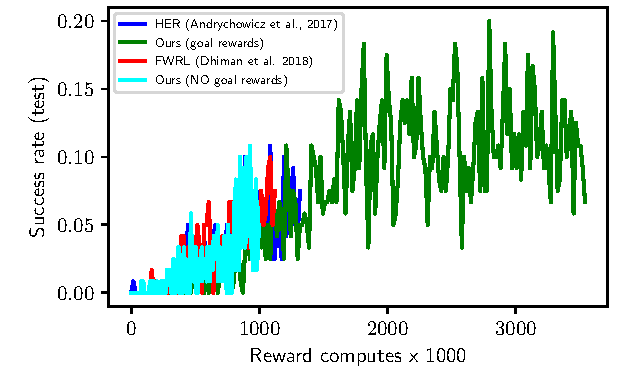
\includegraphics[width=\frac\columnwidth]{media/res/6efc1de-path_reward_low_thresh_chosen-FetchSlidePR-v1-dqst/reward_computes-test/success_rate.pdf}\\
  {.\tiny\color{blue}\hspace{0.8cm}(a) Distance on Epochs \hspace{1.05cm}(b) Distance on
    reward computes
    \hspace{0.70cm} (c) Success rate on epochs \hspace{0.9cm} (d) Success rate on reward computes}
    \caption{For the fetch tasks, we compare our method (red) against HER (blue) ~\citep{andrychowicz2016learning}
    and FWRL (green) ~\citep{dhiman2018floydwarshall} for the distance-from-goal
    and success rate metrics. Furthermore both metrics are plotted
    against two progress measures, the number of training epochs and the number of reward
    computations. Except for the Fetch Slide task, we get comparable or
    better performance across the metrics and progress measures. 
    }%
  \label{fig:fetch-results}%
\end{figure}


\subsection{Hyper-parameters choices}
Unless specified, all our hyper-parameters are identical to the ones
used in the HER
implementation~\citep{dhariwal2017baselines}. We note two main changes
to HER to make the comparison more fair. Firstly,
we use a smaller \emph{distance-threshold}.
The environment used for HER and FWRL returns the goal-reward when the
achieved goal is within this threshold of the desired goal. Because of
the absence of goal-rewards, the distance-threshold information is not used by our
method.
We reduce the it to 1cm which is reduction by a factor of 5 compared to
HER.

Secondly, due to hardware limitations we run all experiments on 6
cores each
while HER uses 19. The batch size used is a function of the number of
cores and hence this parameter has a significant effect on learning. 

However, to ensure fair comparison, all experiments are run with the same hyper-parameters and
random seeds to ensure that variations in performance are purely due
to differences between the algorithms.

\subsection{Results}
% Due to space limitations and in the interest of clarity we show a subset our experiments across both platforms that emphasize both strengths and weaknesses of our algorithm.
All our experimental results are described below. We highlight the strengths and
weaknesses of our algorithm. Across all our experiments, the
distance-to-the-goal metric achieves comparable performance to HER
\emph{without requiring goal-rewards}. 

\paragraph{Fetch Tasks}

The experimental results for Fetch tasks are shown in
Figure~\ref{fig:fetch-results}. For the Fetch Reach and Push tasks our
method achieves comparable performance to the baselines 
across both metrics in terms of training epochs and outperforms them in
terms of reward computations. Notably, the Fetch
Pick and Place trains significantly faster in terms of epochs. For the Fetch
Slide task the opposite is true.
We conjecture that the Fetch-Slide is more sensitive to the
distance-threshold information which our method is unable to use.

\paragraph{Hand Tasks}

For the Hand tasks the distance to the goal and the success rate show different trends.
We show the results in Figure~\ref{fig:hand-results}.
For the distance metric when plotted against epochs, we get comparable
performance for all tasks; when plotted for reward computations we outperform
all baselines except for the Hand Reach tasks. The baselines perform
well enough on this task leaving less scope for significant improvement.
These trends does not hold for the success rate. Our method
consistently under-performs compared to the baselines across tasks. This
is surpising as evidenced by the distance-from-goal metric all the
algorithms are equally far away from the goal on an average. We conjecture that this might be because of
high distance failure cases of the baselines i.e. when the baselines
fail, they do so at larger distances from the goal. In contrast, we
assume our method's success and failiure cases are closer together. 
\begin{figure}
  \def\frac{0.24}
  \rotatebox{90}{{\tiny \hspace{0.5cm} \color{blue}{Hand Reach}}}%
  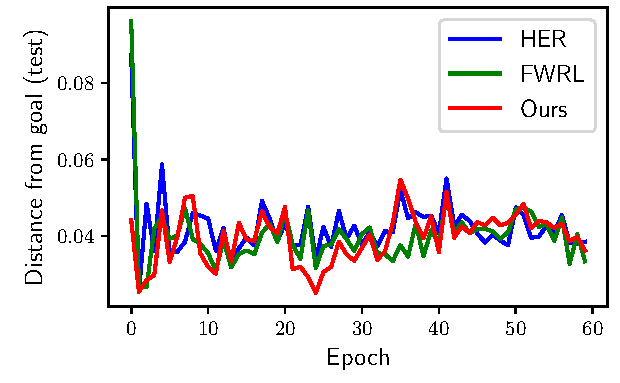
\includegraphics[width=\frac\columnwidth]{media/res/6efc1de-path_reward_low_thresh_chosen-HandReachPR-v0-dqst/epoch-test/ag_g_dist.pdf}%
  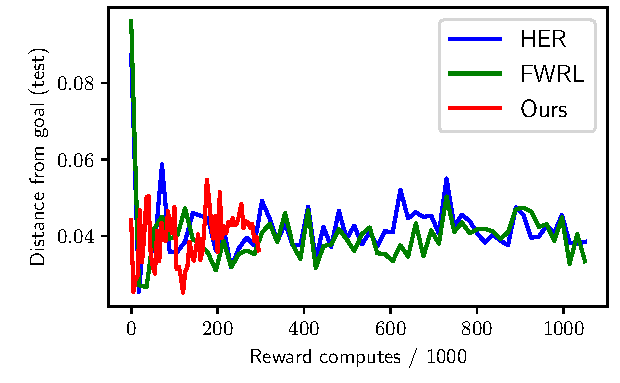
\includegraphics[width=\frac\columnwidth]{media/res/6efc1de-path_reward_low_thresh_chosen-HandReachPR-v0-dqst/reward_computes-test/ag_g_dist.pdf}%
  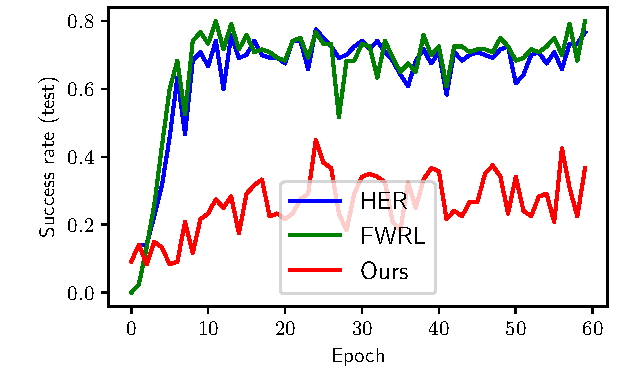
\includegraphics[width=\frac\columnwidth]{media/res/6efc1de-path_reward_low_thresh_chosen-HandReachPR-v0-dqst/epoch-test/success_rate.pdf}%
  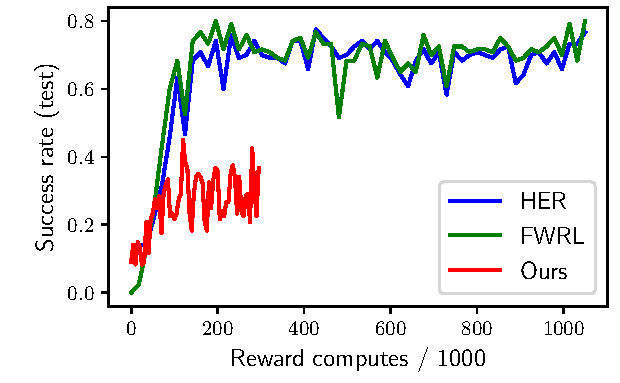
\includegraphics[width=\frac\columnwidth]{media/res/6efc1de-path_reward_low_thresh_chosen-HandReachPR-v0-dqst/reward_computes-test/success_rate.pdf}\\
  \rotatebox{90}{{\tiny \hspace{1em} \color{blue}{Hand Block Rotate}}}%
  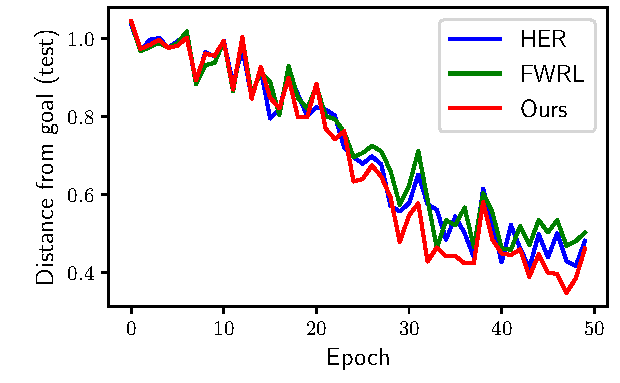
\includegraphics[width=\frac\columnwidth]{media/res/6efc1de-path_reward_low_thresh_chosen-HandManipulateBlockRotateXYZPR-v0-dqst/epoch-test/ag_g_dist.pdf}%
  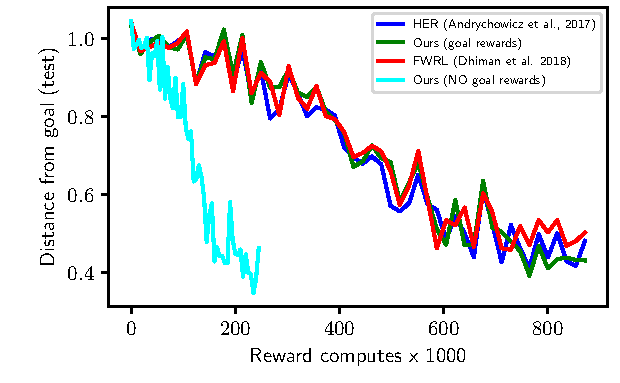
\includegraphics[width=\frac\columnwidth]{media/res/6efc1de-path_reward_low_thresh_chosen-HandManipulateBlockRotateXYZPR-v0-dqst/reward_computes-test/ag_g_dist.pdf}%
  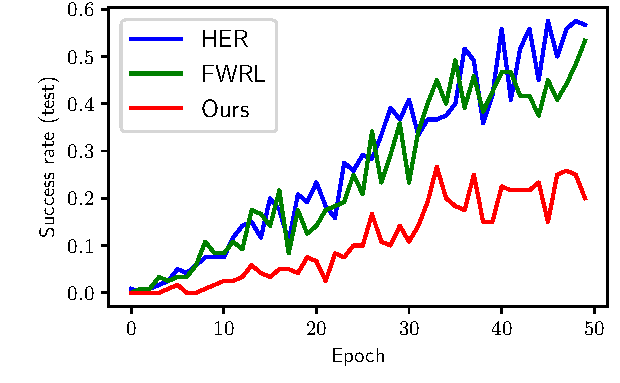
\includegraphics[width=\frac\columnwidth]{media/res/6efc1de-path_reward_low_thresh_chosen-HandManipulateBlockRotateXYZPR-v0-dqst/epoch-test/success_rate.pdf}%
  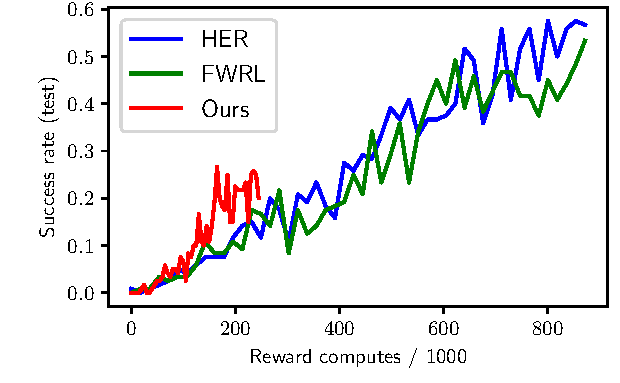
\includegraphics[width=\frac\columnwidth]{media/res/6efc1de-path_reward_low_thresh_chosen-HandManipulateBlockRotateXYZPR-v0-dqst/reward_computes-test/success_rate.pdf}\\
  \rotatebox{90}{{\tiny \hspace{0.7cm} \color{blue}{Hand Egg}}}%
  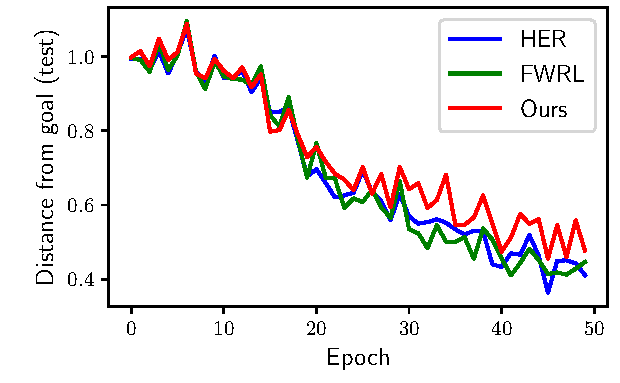
\includegraphics[width=\frac\columnwidth]{media/res/6efc1de-path_reward_low_thresh_chosen-HandManipulateEggFullPR-v0-dqst/epoch-test/ag_g_dist.pdf}%
  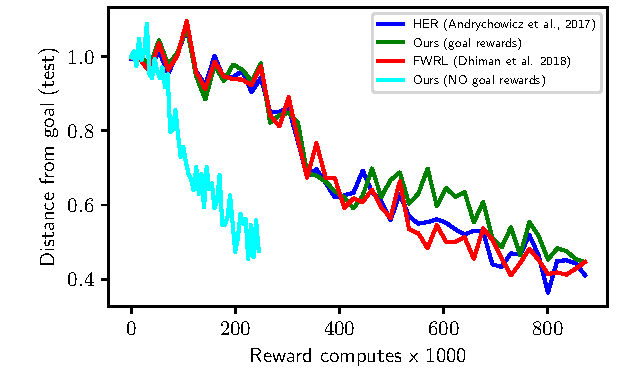
\includegraphics[width=\frac\columnwidth]{media/res/6efc1de-path_reward_low_thresh_chosen-HandManipulateEggFullPR-v0-dqst/reward_computes-test/ag_g_dist.pdf}%
  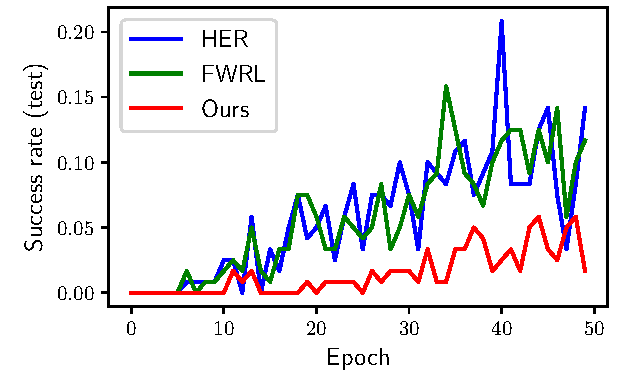
\includegraphics[width=\frac\columnwidth]{media/res/6efc1de-path_reward_low_thresh_chosen-HandManipulateEggFullPR-v0-dqst/epoch-test/success_rate.pdf}%
  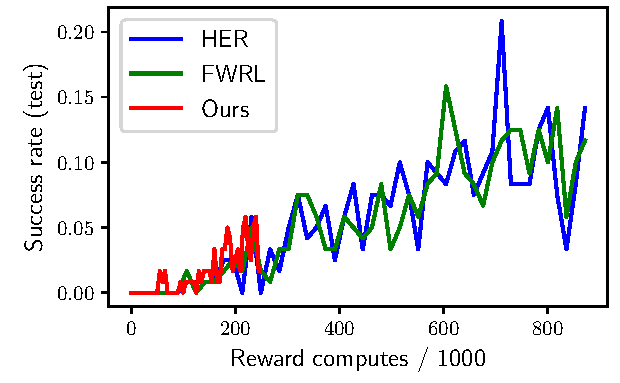
\includegraphics[width=\frac\columnwidth]{media/res/6efc1de-path_reward_low_thresh_chosen-HandManipulateEggFullPR-v0-dqst/reward_computes-test/success_rate.pdf}\\
  \rotatebox{90}{{\tiny \hspace{0.5cm} \color{blue}{Hand Pen Rotate}}}%
  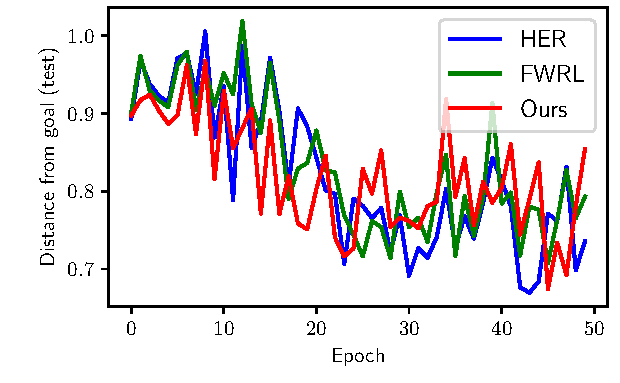
\includegraphics[width=\frac\columnwidth]{media/res/6efc1de-path_reward_low_thresh_chosen-HandManipulatePenRotate-v0-ddpg/epoch-test/ag_g_dist.pdf}%
  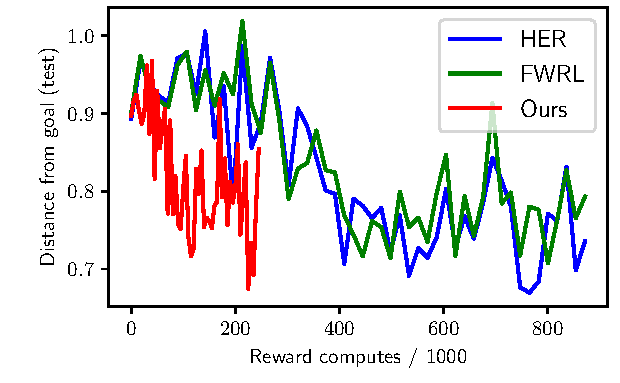
\includegraphics[width=\frac\columnwidth]{media/res/6efc1de-path_reward_low_thresh_chosen-HandManipulatePenRotate-v0-ddpg/reward_computes-test/ag_g_dist.pdf}%
  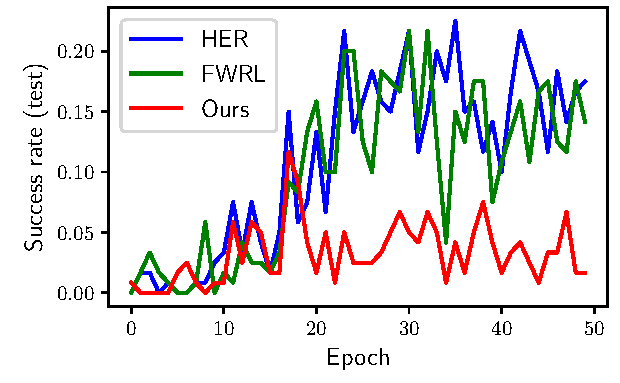
\includegraphics[width=\frac\columnwidth]{media/res/6efc1de-path_reward_low_thresh_chosen-HandManipulatePenRotate-v0-ddpg/epoch-test/success_rate.pdf}%
  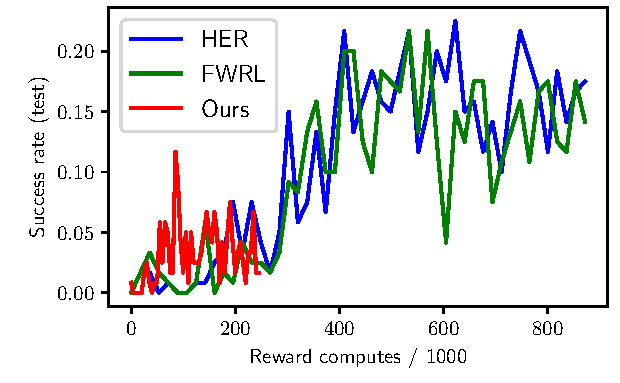
\includegraphics[width=\frac\columnwidth]{media/res/6efc1de-path_reward_low_thresh_chosen-HandManipulatePenRotate-v0-ddpg/reward_computes-test/success_rate.pdf}
  {.\tiny\color{blue}\hspace{0.8cm}(a) Distance on Epochs \hspace{1.05cm}(b) Distance on
    reward computes
    \hspace{0.70cm} (c) Success rate on epochs \hspace{0.9cm} (d) Success rate on reward computes}
  \caption{For the hand tasks, we compare our method (red) against HER (blue) ~\citep{andrychowicz2016learning}
    and FWRL (green) ~\citep{dhiman2018floydwarshall} for the distance-from-goal
    and success rate metrics. Furthermore, both metrics are plotted
    against two progress measures, the number of training epochs and the number of reward
    computations. Measured by distance from the goal, our method performs comparable to or
    better than the baselines for both progress measurements. For the success rate,
    our method underperforms against the baselines. 
}%
  \label{fig:hand-results}%
\end{figure}%
% 

